\chapter[Scoring \& Classification Sectorielle]{Réalisation : Moteur de Scoring \& Classification Sectorielle}
\label{chap:scoring}

\section{Algorithme Mathématique de Scoring Pondéré}
L'agrégation des résultats d'audit repose sur un modèle mathématique à coefficients pondérés inspiré des meilleures pratiques internationales, mais calibré sur les priorités défensives de l'administration tunisienne.

\subsection{Formule de Calcul}
Soit $N = 16$ l'ensemble des facteurs de risque audités. Pour chaque catégorie $i \in \{1, \dots, N\}$, on note $S_i \in [0, 100]$ le score partiel obtenu et $w_i \in ]0, 1]$ son coefficient de pondération respectif, tel que $\sum_{i=1}^{N} w_i = 1.0$.

Le score global de cybersécurité de l'organisme audité, noté $\text{Score}_{\text{global}} \in [0, 100]$, est défini par la combinaison linéaire normalisée suivante :
\begin{equation}
\text{Score}_{\text{global}} = \sum_{i=1}^{N} \left( w_i \times S_i \right) - \sum_{k \in \mathcal{V}_{\text{critique}}} \mathcal{P}_k
\end{equation}
où $\mathcal{V}_{\text{critique}}$ représente l'ensemble des vulnérabilités critiques rédhibitoires détectées (ex: injection SQL avérée, port de base de données exposé sur Internet sans pare-feu, certificat SSL révoqué), et $\mathcal{P}_k$ une pénalité de sévérité directe (fixée à 15 points par défaut).

\subsection{Grille de Pondération des 16 Facteurs d'Évaluation}
La distribution des poids reflète la criticité opérationnelle des vecteurs d'attaque :

\begin{table}[!htbp]
\centering
\caption{Grille de pondération des 16 facteurs d'audit de CyberScore TN}
\label{tab:weights}
\begin{singlespace}
\footnotesize
\renewcommand{\arraystretch}{1.0}
\begin{tabularx}{\textwidth}{p{4.6cm} c c X}
\toprule
\textbf{Facteur de Risque Audité} & \textbf{Poids} & \textbf{Pts} & \textbf{Justification Opérationnelle} \\
\midrule
Vulnérabilités Web (OWASP ZAP) & 0.15 & 15 & Risque direct d'injections SQL et de compromission. \\
Chiffrement SSL / TLS \& Ciphers & 0.12 & 12 & Confidentialité des flux d'échange citoyen-État. \\
En-têtes HTTP (HSTS / CSP) & 0.10 & 10 & Barrière défensive primaire du navigateur contre les attaques. \\
Sécurité DNS \& DNSSEC & 0.08 & 8 & Protection contre le détournement de trafic et cache poisoning. \\
Exposition Réseau (Ports Nmap) & 0.08 & 8 & Réduction de la surface d'accès aux services internes. \\
Sécurité Email (SPF / DMARC) & 0.06 & 6 & Lutte contre l'usurpation ministérielle et le phishing. \\
Content Security Policy (CSP) & 0.06 & 6 & Atténuation stricte des attaques Cross-Site Scripting (XSS). \\
Sécurité Cookies de Session & 0.05 & 5 & Protection contre le vol de session et détournement. \\
Supply Chain \& CDN (SRI) & 0.05 & 5 & Prévention des attaques par rebond sur dépendances tierces. \\
Fuite d'Infos Techniques (\texttt{.git}) & 0.05 & 5 & Masquage de la topologie interne et des versions serveurs. \\
Surface d'Attaque EASM & 0.04 & 4 & Détection des serveurs fantômes et environnements oubliés. \\
Réputation CTI (Threat Intel) & 0.04 & 4 & Détection des adresses IP compromises et listes noires. \\
Obsolescence des Technologies & 0.03 & 3 & Identification des versions de CMS et logiciels non patchés. \\
Chaîne de Confiance TunTrust & 0.03 & 3 & Souveraineté de l'autorité de certification nationale. \\
Protection Données Privées & 0.03 & 3 & Garantie de non-exposition des données personnelles. \\
Conformité Décret 2023-17 & 0.03 & 3 & Alignement formel sur les directives de sécurité ANCS. \\
\midrule
\textbf{Total National} & \textbf{1.00} & \textbf{100} & \textbf{Évaluation Complète de la Posture Souveraine} \\
\bottomrule
\end{tabularx}
\end{singlespace}
\end{table}

\section{Système de Notation Duale}
Pour répondre à la fois au besoin technique des officiers RSSI et au besoin décisionnel des ministres et directeurs généraux, CyberScore TN propose une notation duale :

\begin{table}[!htbp]
\centering
\caption{Grille de correspondance des Notes, Grades alphabétiques et Étoiles}
\label{tab:grades}
\begin{singlespace}
\footnotesize
\renewcommand{\arraystretch}{1.1}
\begin{tabularx}{\textwidth}{c c c c X}
\toprule
\textbf{Plage de Score} & \textbf{Grade} & \textbf{Étoiles} & \textbf{Mention Officielle} & \textbf{Signification Opérationnelle} \\
\midrule
$95 - 100$ & \textbf{A+} & $\star\star\star$ & Exemplaire & Posture de sécurité optimale, TLS 1.3 et DNSSEC actifs. \\
$90 - 94$  & \textbf{A}  & $\star\star\star$ & Excellent & Très haut niveau de cyber-hygiène, 0 alerte critique. \\
$80 - 89$  & \textbf{B}  & $\star\star\star$ & Bon & Bon niveau global, quelques optimisations recommandées. \\
$70 - 79$  & \textbf{C}  & $\star\star\phantom{\star}$ & Acceptable & Conforme aux standards de base, carences sur HSTS ou CSP. \\
$60 - 69$  & \textbf{D}  & $\star\phantom{\star\star}$ & Insuffisant & Vulnérabilités moyennes nombreuses, remédiation sous 30 jours. \\
$0 - 59$   & \textbf{F}  & $\star\phantom{\star\star}$ & Critique & Présence d'alertes critiques actives, intervention immédiate. \\
\bottomrule
\end{tabularx}
\end{singlespace}
\end{table}

\section{Classification Sectorielle des Organismes Publics Tunisiens}
Afin de structurer le monitoring national, CyberScore TN classe l'ensemble du patrimoine numérique de l'État en quatre secteurs d'activité administrative :
\begin{enumerate}
    \item \textbf{Ministères (24 départements)} : Départements ministériels centraux (\texttt{finances.gov.tn}, \texttt{interieur.gov.tn}, \texttt{defense.nat.tn}, etc.).
    \item \textbf{Institutions Publiques (25+ agences)} : Instances constitutionnelles, agences nationales et régulateurs (\texttt{ancs.tn}, \texttt{bct.gov.tn}, \texttt{isie.tn}, etc.).
    \item \textbf{Collectivités Locales (50+ collectivités)} : Gouvernorats régionaux et municipalités (\texttt{commune-tunis.gov.tn}, \texttt{commune-sfax.gov.tn}, etc.).
    \item \textbf{Entreprises Publiques (20+ sociétés)} : Sociétés d'État et offices publics (\texttt{steg.com.tn}, \texttt{sonede.com.tn}, \texttt{poste.tn}, etc.).
\end{enumerate}

La Figure \ref{fig:benchmark_view} illustre le tableau de bord comparatif permettant à l'ANCS de suivre le niveau moyen de conformité par secteur et d'identifier les organismes nécessitant un appui prioritaire.

\begin{figure}[!htbp]
\centering
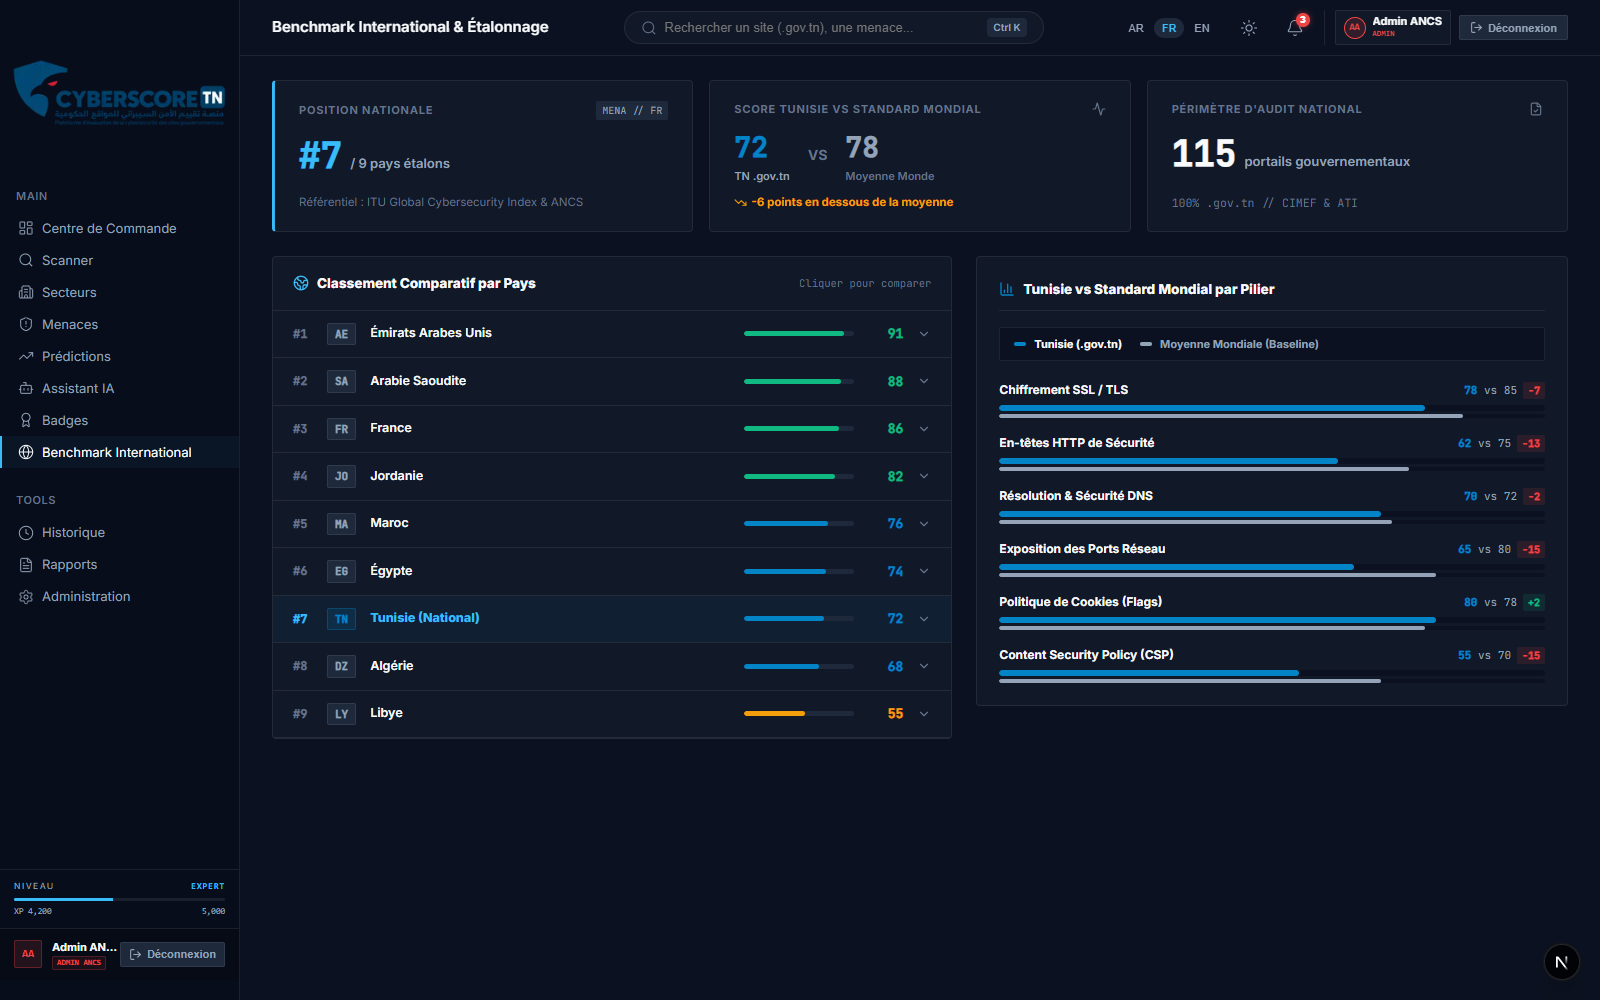
\includegraphics[width=0.70\textwidth]{images/benchmark.png}
\caption{Observatoire comparatif et benchmark sectoriel des institutions d'État}
\label{fig:benchmark_view}
\end{figure}

\section{Modélisation Prédictive des Risques à +30 Jours}
Le moteur analytique corrèle l'historique temporel des audits avec les cycles d'expiration des certificats X.509 et les délais moyens de remédiation observés pour projeter la note de chaque institution à horizon 30 jours (Figure \ref{fig:predictions_view}).

\begin{figure}[!htbp]
\centering
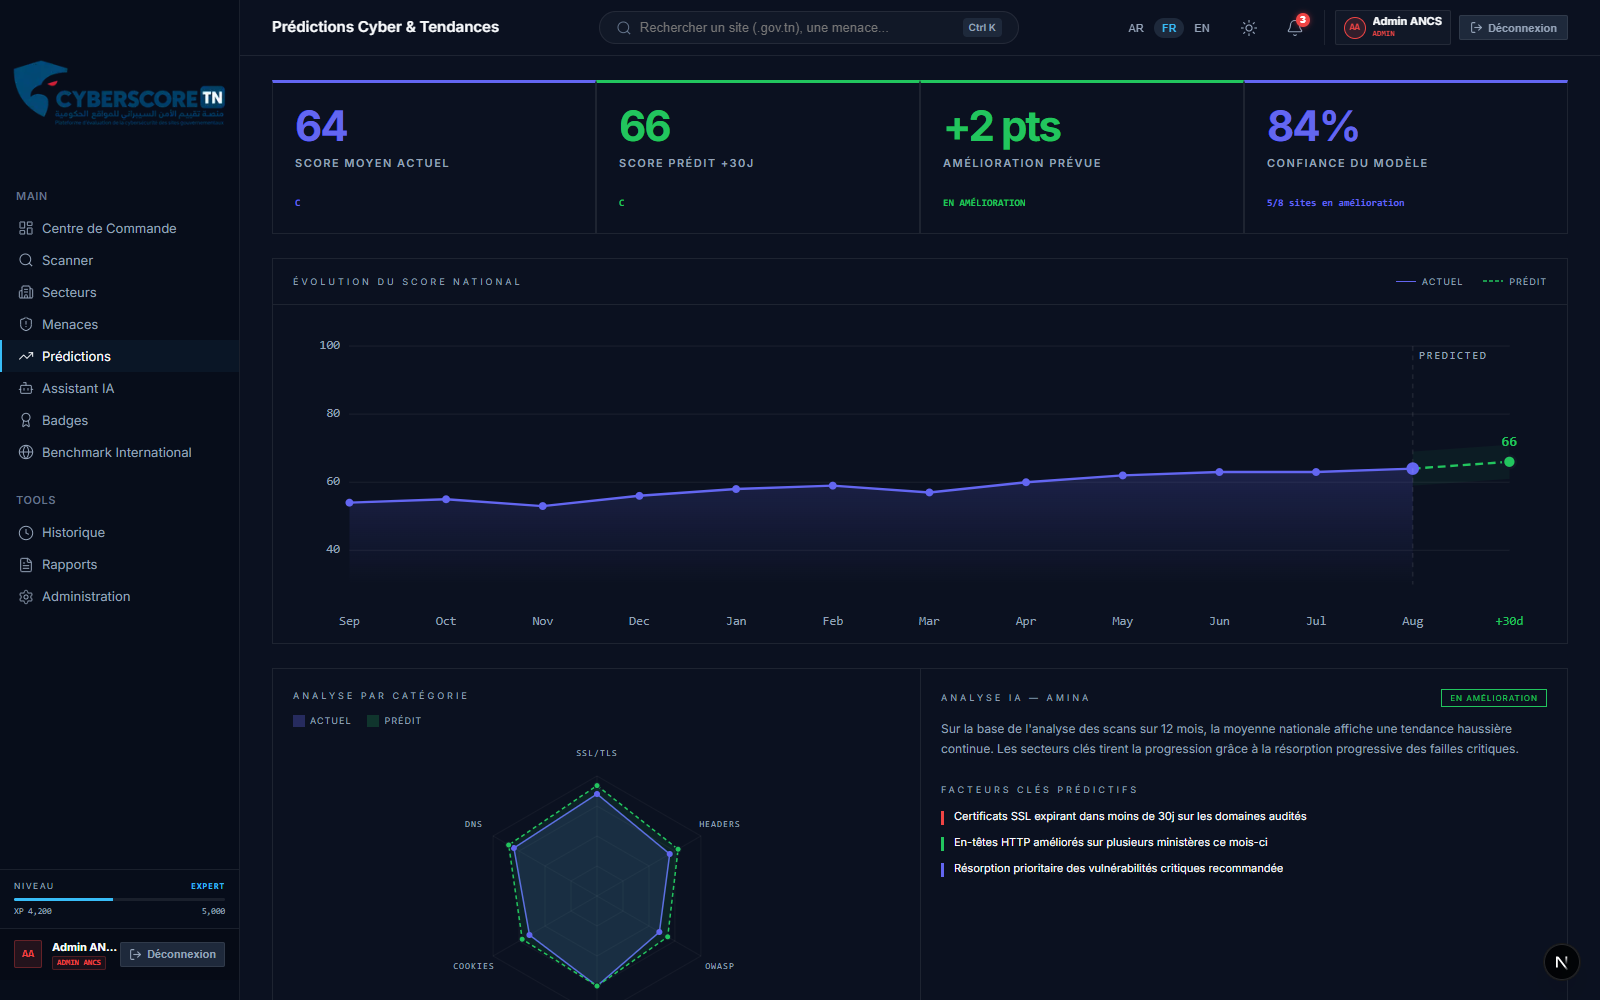
\includegraphics[width=0.70\textwidth]{images/predictions.png}
\caption{Module d'analyse prédictive et projections de dérive de score à +30 jours}
\label{fig:predictions_view}
\end{figure}
